
\setcounter{page}{1}
\section{Zielsetzung}
Ziel dieses Versuchs ist die Bestimmung unbekannter Widerstände,
Induktivitäten und Kapazitäten.
Dies geschieht mit Hilfe von elektrischen Brückenschaltungen.
\section{Theorie}
Eine allgemeine Brückenschaltung ist in Abbildung (\ref{fig:br}) zu sehen.

\begin{figure}
  \centering
  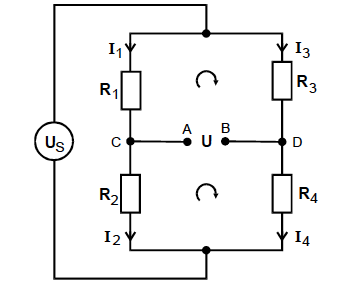
\includegraphics[scale = 0.7]{Bruecke1.PNG}
  \caption{Prinzipielle Brückenschaltung\protect\cite{on3}}
  \label{fig:br}
\end{figure}
Mit solch einer Brückenschaltung wird eine Potentialdifferenz untersucht.
Zwischen den Punkten A und B tritt eine Brückenspannung auf.
Zur Berechnung dieser Spannung werden die beiden Kirchhoffschen Gesetze verwendet
\begin{align}
  \sum_k I_k &= 0 \\
  \sum_k U_k &= 0
\end{align}
Diese sagen aus, dass die in einem Knoten hineinlaufenden Ströme, gleich der hinauslaufenden Ströme sein müssen.
Außerdem muss in einer Masche die Summe aller Spannungen gleich Null sein.
Aus den Kirchhoffschen Regeln und der Formel für die Speisespannung,
\begin{equation}
  U_s = I_1(R_1 + R_2)
\end{equation}
ergibt sich nun ein Zusammenhang für die Brückenspannung in Abhängigkeit von den Schaltungsparametern.
\begin{equation}
  U = \frac{R_2R_3 - R_1R_4}{(R_3+R_4)(R_1+R_2)}\cdot U_s
\end{equation}
Die Brückenschaltung gilt als abgeglichen, wenn
\begin{equation}
R_1R_4=R_2R_3
\label{eqn:1}
\end{equation}
gilt.

\subsection{Wheatstone`sche Brückenschaltung}
Die Wheatstone`sche Brückenschaltung dient zur Bestimmung eines unbekannten Widerstandes $R_x$.
Der Aufbau einer solchen Brückenschaltung ist in Abbildung (\ref{fig:whe}) zu sehen.
\begin{figure}
  \centering
  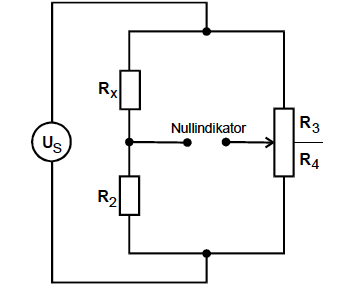
\includegraphics[scale = 0.7]{Wheat.PNG}
  \caption{Wheatstone Brückenschaltung\protect\cite{on3}}
  \label{fig:whe}
\end{figure}
Da die Schaltung nur von Widerständen abhängt,
kann sie sowohl im wechselstrom als auch im Gleichstrom betrieben werden.
Es ist nur wichtig den Nullindikator passend zu wählen.
Der unbekannte Widerstand kann wegen (\ref{eqn:1}) durch
\begin{equation}
  R_x = \frac{R_2R_3}{R_4}\, .
\end{equation}
bestimmt werden.

\subsection{Kapazitätsmessbrücke}
Zur Bestimmung eines unbekannten kondensators, eignet sich ein Aufbau
wie er in Abbildung (\ref{fig:kapa}) zu sehen ist.
\begin{figure}
  \centering
  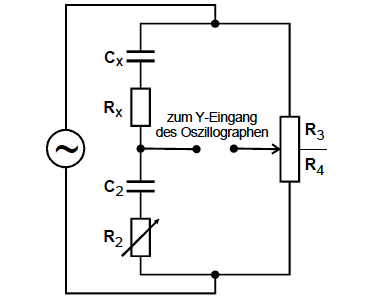
\includegraphics[scale = 0.7]{Kapa.PNG}
  \caption{Kapazitätsmessbrücke\protect\cite{on3}}
  \label{fig:kapa}
\end{figure}
Ein realer Kondensator wandelt hindurchfließende elektrische Energie zum Teil in Wärme um.
Der komplexe Widerstand eines solchen Kondensators lauten somit:
\begin{equation*}
  Z = R - \frac{i}{\omega C}
\end{equation*}
Hinter dem unbekannten Kondensator ist ein unbekannter Widerstand geschaltet,
der eine Phasenverschiebung verursachen würde,
weshalb zweivoneinander unabhängige veränderliche Widerstände eingebaut werden müssen.
Die Formeln für den unbekannten Widerstand und Kondensator lauten:
\begin{align}
  R_x &= \frac{R_2R_3}{R_4} \\
  C_x &= \frac{C_2R_4}{R_3}
\end{align}

\subsection{Induktivitätsmessbrücke}
Im der folgenen Abbildung (\ref{fig:indu}) ist eine Schaltung gezeigt,
mit der eine unbekannte Spule bestimmt werden kann.
\begin{figure}
  \centering
  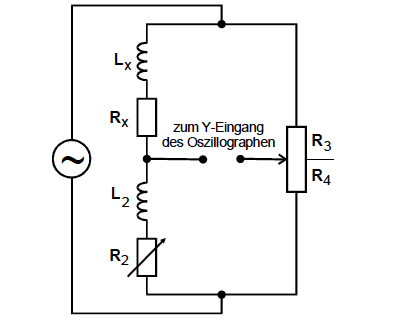
\includegraphics[scale = 0.7]{Indu.PNG}
  \caption{Induktivitätsmessbrücke\protect\cite{on3}}
  \label{fig:indu}
\end{figure}
Eine reale Indutivität wandelt einen Teil der magnetischen Feldenergie in Wärme um.
Hier lautet der komplexe Widerstand:
\begin{equation*}
  Z = R + i\omega L
\end{equation*}
Somit ergeben sich nun die Formeln
\begin{align}
  R_x &= \frac{R_2R_3}{R_4} \\
  L_x &= \frac{L_2R_3}{R_4}
\end{align}
für den Unbekannten Widerstand und die Spule.

\subsection{Maxwell-Brücke}

Mit der Mawellbrüce ist es ebenfalls möglich eine unbekannte Induktivität zu bestimmen.
Sie hat den Vorteil, dass auf eine bekannte Induktivität verzichtet werden kann.
Dafür wird eine Kapazität eingebaut, die einen deutlich geringeren Wirkwiderstand hat.
\begin{figure}
  \centering
  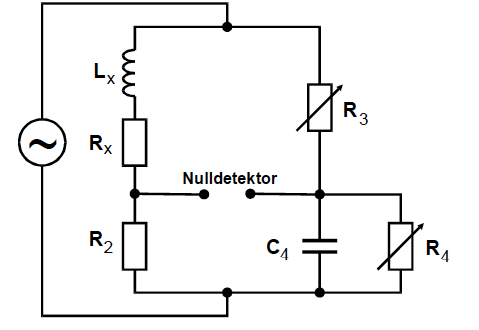
\includegraphics[scale = 0.7]{Max.PNG}
  \caption{Induktivitätsmessbrücke\protect\cite{on3}}
  \label{fig:max}
\end{figure}
Für die unbekannte Induktivität gilt:
\begin{equation*}
  Z_x = R_x +i\omega L_x\cdot \frac{1}{Z_4}
\end{equation*}
Für den Kondensator gilt
\begin{equation*}
  \frac{1}{Z_4} = \frac{1}{R_4} + i\omega \cdot C_4 \, .
\end{equation*}
Mit dieser Überlegung ergeben sich die Formeln:
\begin{align}
  R_x &= \frac{R_2R_3}{R_4} \\
  L_x &= R_2R_3C_4
\end{align}

\subsection{Wien-Robinson-Brücke}
In dieser Brücke sind keine Unbekannten Bauteile.
Sie ist im Gegensatz zu den anderen Brücken Frequenzabhängig.
Eine beispielhafte Abbildung ist in (\ref{fig:wien}) zu sehen.

\begin{figure}
  \centering
  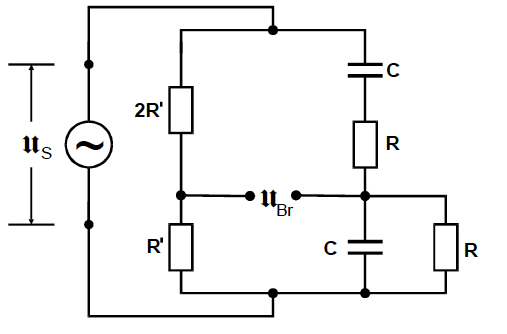
\includegraphics[scale = 0.7]{Wien.PNG}
  \caption{Wien-Robinson-Brücke\protect\cite{on3}}
  \label{fig:wien}
\end{figure}
Es wird das Verhältnis der Brückenspannung zur Speisespannung betrachtet:
\begin{equation}
  \left|\frac{U_{Br}}{U_s}\right|^2 = \frac{1}{9}\cdot \frac{(\Omega - 1)^2}{(1- \Omega)^2 + 9\Omega ^2}
  \label{eqn:WiRo}
\end{equation}
Dabei ist
\begin{equation*}
  \Omega = \frac{\omega}{\omega_0}
\end{equation*}
und
\begin{equation}
  \omega = \frac{1}{RC}
  \label{eqn:aus}
\end{equation}
Bei dem Verhältnis in (\ref{eqn:aus}) verschwindet die Brückenspannung
und die Brücke ist ausgeglichen.
Die Wien-Robinson-Brücke dient als frequenzfilter.
